\documentclass[letterpaper,onecolumn,titlepage]{Ythesis}

\usepackage[utf8]{inputenc}
\usepackage{tikz}
\usetikzlibrary{mindmap}
\usetikzlibrary{arrows.meta, chains, positioning, shapes.geometric}


\usepackage{graphicx}
\graphicspath{{sections/figs/}{.figs/}}

\usepackage[backend=bibtex, style=numeric-comp]{biblatex}
\bibliography{glasslab_viz}

\usepackage{array,multirow,graphicx}
\usepackage{subcaption}
\usepackage{subfiles}
\usepackage{url}
\usepackage{amsmath}
\usepackage{float}

\title{Visualizing Conditional Dependencies}
\author{Hannah Aizenman}
\committee{Dr. Michael Grossberg (Advisor), Dr. Robert Haralick, Dr. Lev Manovich, Dr. Huy Vo}
\submitted{}
\abstract{Often the question in data exploration is not if a pattern occurs, but why. The search for the why is often the search for a conditionally dependent relationship in the dataset. While there are visualization methods that can be used to uncover a potential causal link between variables in the dataset, many of these techniques only work when the causal variables are categorical or can only be applied between two variables at a time or discard the complex, often spatiotemporal, structure of the dataset. Instead structure preserving methods for visualizing the distribution of observations provide a way of understanding some of the probabilistic relationships within and between the observations in these complex datasets. Using the type and structure of the variables in a dataset as a guide, this survey presents methods for visualizing conditional dependencies for multivariate datasets with discrete observations and visualizing probability distributions for datasets where observations are drawn from a continuous (functional) space. Because there is limited literature on explicit ways to visualize conditional dependency, we include techniques that suggest or can be adapted to show these dependencies.}

\begin{document}
\makefrontmatter

\section{Introduction}
\label{sec:introduction}
Data visualization can reveal complex relationships in datasets that are not apparent from the descriptive statistical summary\cite{anscombe_graphs_1973}. It can be useful to model the variables of a dataset as random variables and explore the probability distributions of those variables, but that is also a more challenging visualization task. Many observed relationships are not explicit functional dependencies of variables but instead may be expressed in terms of a probabilistic relationship between random variables. For example, a street vendor may want to sell umbrellas. They notice that the people who already have umbrellas tend to be wearing coats. So should they target people without coats? Maybe, but only in that someone who is unprepared for the weather in one way is also likely to be unprepared in other ways. So the intervention only make sense on days when the underlying condition for needing the coat and umbrella is present-namely it is raining. Being able to visualize that conditional dependence greatly aides in potentially finding it. 

\begin{figure}[H]
	\center
	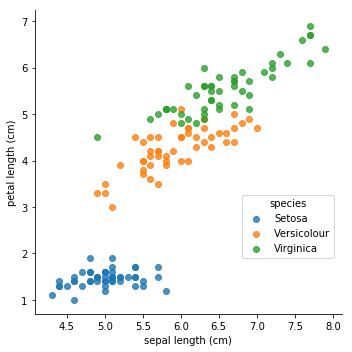
\includegraphics[width=1\textwidth]{intro/iris_scatter.png}
  	\caption{Pairwise relationship between Iris sepal length and Iris petal length (cm) in the Iris scikit-learn dataset\cite{scikit-learn}.}
  	\label{fig:iris_scatter}
\end{figure}

To understand how to visualize that conditional dependency, we need to talk about visualizations in a formal manner. To introduce the visualization terminology used throughout this paper, we use the Iris flower dataset \cite{fisher_use_1936-1, _uci_????} distributed with the scikit-learn Python machine learning library \cite{scikit-learn}. The Iris dataset has 150 observations that have a categorical species attribute and quantitative sepal length, sepal width, petal length, and petal width attributes. We start probing the Iris dataset for conditional dependencies with the scatter plot in figure~\ref{fig:iris_scatter}. The lack of correlation between the petal and length for the Setosa Iris in figure~\ref{fig:iris_scatter}, despite being tightly clustered, indicates that petal and sepal length are dependent on the species of Iris being Setosa. While a scatter plot may work for 2 quantitative variables and a relatively small number of data points, even trying to visualize all the variables of the Iris dataset pushes against the limits of the scatter plot. This survey will discuss some methods for addressing the challenges of large and complex datasets, but first we must review some visualization terminology. 

\subsection{Terminology}
\begin{figure}[H]
\begin{tikzpicture}[
    node distance = 5mm and 7mm,
      start chain = going right,
 disc/.style = {shape=cylinder, draw, shape aspect=0.3,
                shape border rotate=90,
                text width=17mm, align=center, font=\linespread{0.8}\selectfont},
  mdl/.style = {shape=ellipse, aspect=2.2, draw},
  alg/.style = {draw, align=center, font=\linespread{0.8}\selectfont}
                    ]
    \begin{scope}[every node/.append style={on chain, join=by -Stealth}]
\node (n1) [disc, minimum width=3cm] {Dataset};
\node (n2) [alg]  {Invariant};
\node (n4) [disc, minimum width=3cm] {Components};
    \end{scope}
\node(n5)[above right=of n4, xshift=2cm, inner sep=0pt] {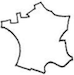
\includegraphics[width=.2\textwidth]{sections/figs/intro/catquant}};
\node(n6)[below right=of n4, xshift=2cm, inner sep=0pt] {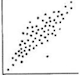
\includegraphics[width=.2\textwidth]{sections/figs/intro/quantquant.png}};

\draw[->] (n4) -- (n5);
\draw[->] (n4) -- (n6);
\end{tikzpicture}

\caption{To go from a dataset to a visualization, the data is subset based on a set of constraints (the invariant). The resulting subset becomes the components that are visualized, but the choice of visualization is dependent on the type and structure of the component variables.}
\label{fig:flowchart}
\end{figure}

Given a dataset, we need to decide what subset of the data to visualize. Bertin describes the set of constraints used to subset the data as the \textit{invariant}. Formally, the \textit{invariant} is the set of shared characteristics of the data being visualized. When these constraints are applied to the dataset, the resulting subset is what will become the \textit{components} of the visualization \cite{bertin_semiology_2011}. In figure~\ref{fig:iris_scatter}, the \textit{invariant} common to all the data being visualized is "sepal length", "petal length", and "species" and the \textit{components} are the measurements of these variables. As shown in figure~\ref{fig:flowchart}, the final step in creating a visualization is choosing how to encode the
components using retinal (visual) variables.
 

\subsubsection{Retinal (Visual) Variables}
\begin{figure}[H]
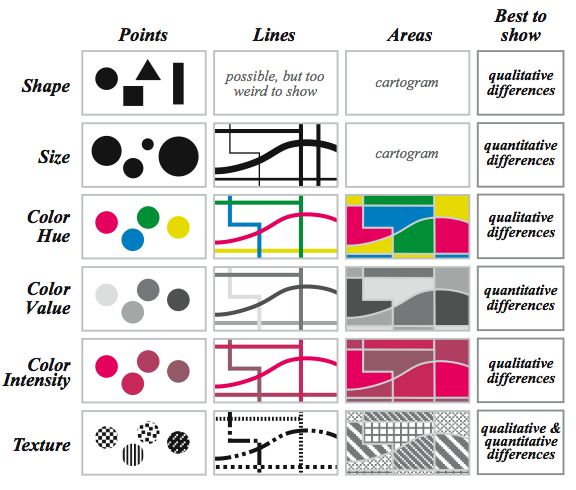
\includegraphics[width=1\textwidth]{intro/retinal_variables.png}
\caption{Retinal variables are a codification of how position, size, shape, color and texture are used to illustrate variations in the \textit{components} of a visualization. This tabular form of Bertin's retinal variables is from Understanding Graphics \cite{_information_????} who reproduced it from \textit{Making Maps: A Visual Guide to Map Design for GIS} \cite{krygier_making_2005}}
\label{fig:retinal_variables}
\end{figure}

Figure~\ref{fig:retinal_variables} illustrates common guidelines for encoding \textit{components}, derived from what Bertin terms a retinal variable and most other visualization theorists call visual variables \cite{bertin_semiology_2011,krygier_making_2005,chambers_graphical_1983,wilkinson_grammar_2005,munzner_visualization_2014}. The columns of figure~\ref{fig:retinal_variables} correspond to the type of observation: discrete points, continuous events (e.g. a timeseries), two dimensional continuous events (e.g. a vector map). The rows of figure~\ref{fig:retinal_variables} describe ways to visualize variations in the \textit{components}; generally, quantitative components are represented by retinal variables that change quantitatively and categorical components are represented by retinal variables that vary qualitatively. In figure~\ref{fig:iris_scatter}, the hue of the marker is used to encode differentiation in species and the position of the marker is used to show variation in petal length and sepal length. The retinal variables suggest that any single visualization is limited to encoding at most about 8 or 9 components. Retinal variables provide guidelines for encoding \textit{components}, but the choice of graph is based on the type and structure of the data. 

\subsubsection{Data Type and Structure}

\begin{figure}[H]
 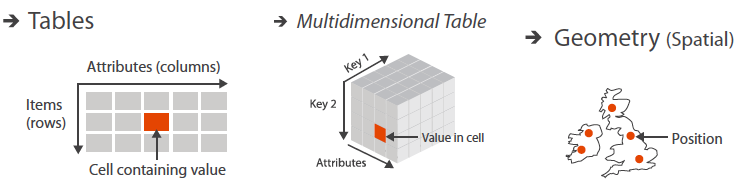
\includegraphics[width=\textwidth]{intro/munzner_datatypes}
\caption{Keys are unique lookup values used to find individual observations in the dataset. Keys are positional references, and can be coordinates on a map or unique values such as a primary key in a database or a (time, latitude, longitude) index in a data cube. Image modified from a diagram from Munzner's website \cite{_visualization_????}}
\label{fig:munzner_datatypes}
\end{figure}

As shown in figure~\ref{fig:flowchart}, there are multiple ways to translate data into pictures. A map is always an option, except when the observations do not have associated coordinates in a physical plane. Tamara Munzner provides a way to distinguish between these datasets using $\{key, value\}$ designations \cite{munzner_visualization_2014}. Munzner defines \textit{values} as measurements of interest in the dataset, analogous to dependent variables in statistics. She defines \textit{keys} as indexes that can be used to look up values, analogous to independent variables in statistics and dimensions in computer science. Figure~\ref{fig:munzner_datatypes} illustrates how these keys are used to look up variables in a dataset: 
\begin{itemize}
	\item map: keys are the coordinates of the points
	\item table: row index, database primary key
	\item data cube: row, column, etc. (.e.g. $i,j,k$) index
\end{itemize}

Expanding on Munzner's key and value semantics, in many datasets the keys are discrete variables like time or geophysical locations sampled from a continuous curve, surface, or field. While these observations are discrete samples from the continuous space, often the continuous (functional) characteristic\cite{ramsay_functional_2006,muller_functional_2006} of the observational space is also of interest. Besides quantitative discrete, quantitative continuous, or categorical measurement type considerations, the choice of visualization is also influenced by the measurement being on an interval, ratio, nominal, or categorical scale. 

\subsubsection{Conditional Probability}
\begin{figure}[H]
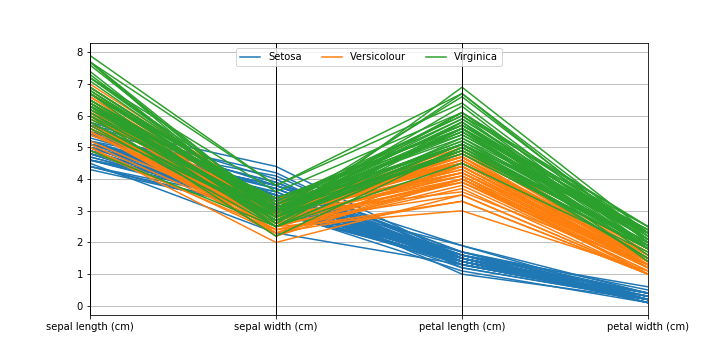
\includegraphics[width=\textwidth]{intro/iris_parallel}
\caption{The parallel coordinates plot (PCP) of the Iris dataset shows the pairwise relationship between adjacent variables. The relative widths of each band of color and the similarities in shape of the orange and green (Iris Versicolour and Iris Virginica) bands and the consistent downward trend amongst the blue (Iris Setosa) bands show how the observations distribute across the species. If the visualization only showed one species, this would be the conditional probability of the multivariate observation given that species.}
\label{fig:iris_parallel}
\end{figure}

Since the Iris dataset has no geographic or temporal components, we do not need to consider techniques designed to preserve map or time semantics. Instead, in figure~\ref{fig:iris_parallel} we plot how the variables in the Iris dataset are related to each other using the the parallel coordinates plot (PCP) \cite{claessen_flexible_2011,_nist/sematech_????,inselberg_plane_1985, wegman_hyperdimensional_1990}. In figure~\ref{fig:iris_parallel}, each line is an observation in the dataset and each color maps to a species of Iris. The color coding then allows for this visualization to be used to show how the four quantitative variables (sepal length, sepal width, petal length, and petal width) distribute within each variable. If we filter the Iris dataset such that we are only looking at one species, then the parallel coordinates plot is visualizing the conditional probability:
\begin{equation}
P(A\mid B) = \frac{P(A \cap B}{P(B)} 
\end{equation}

where A is the observation vector $\left< \text{sepal length, sepal width, petal length, petal width} \right>$ and B is the species of petal. 

\subsubsection{Conditional Dependency}
\label{sec:condep}
\begin{figure}[H]
\center
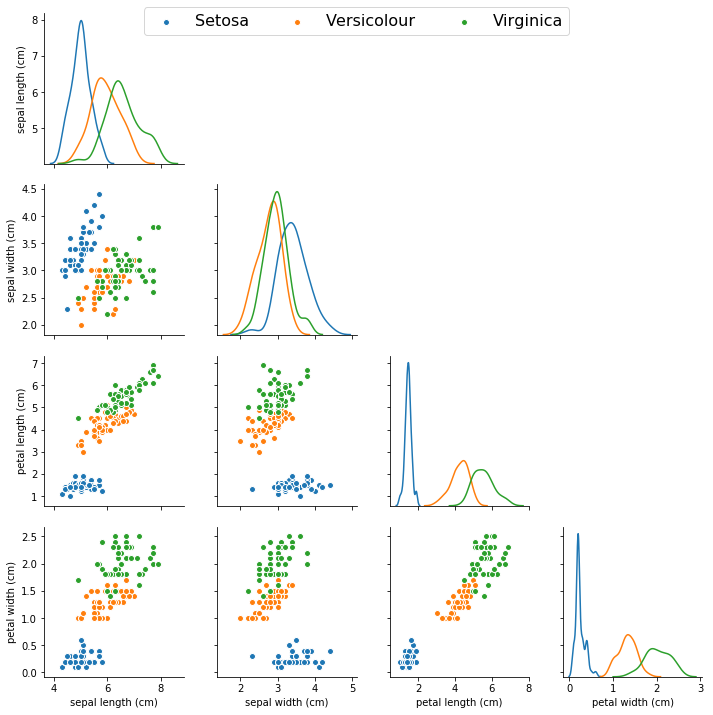
\includegraphics[width=1\textwidth]{intro/iris_observations.png}
\caption{The scatter matrix shows the pairwise relationships color coded by Iris species. The clustering of the (blue) Setosa Iris measurements even when the measurements are not correlated suggests a conditional dependence on species type.}
\label{fig:iris_observations}
\end{figure}
After observing a relationship between Iris variables in figure~\ref{fig:iris_scatter}, we want to learn if there is an underlying reason for the cooccurence of the the variables. The matrix of scatter plots \cite{elmqvist_rolling_2008,l._wilkinson_high-dimensional_2006} in figure~\ref{fig:iris_observations} provides a lot of information about the distribution of variables in the dataset. 
The diagonal of the scatter matrix shows the kernal density estimation (KDE) \cite{scott_multivariate_1992, chambers_graphical_1983, stigler_mathematical_1978} of the distribution of each variable relative to the species type. If the KDE plots are filtered by species type, then this visualization illustrates the conditional probability of each variable relative to a type of species. The scatter matrix plot also shows every set of pairwise relationships in the dataset, color code by Iris species. Because the scatter matrix shows the cooccurence of two variables and is encoded with information about a third variable, it works well as a tool to explore a potential conditional dependency amongst the variables in the dataset \cite{dawid_conditional_1979}. As seen in figure~\ref{fig:iris_observations}, the  measurements of sepal width, sepal length, petal width, and petal length are correlated for Versicolour and Virginica Irises but not for Setosa Irises. Despite the lack of correlation, sepal width, sepal length, petal width, and petal length are tightly clustered for Setosa Irises; this clustering indicates that these quantitative measurements are conditionally dependent on species. The scatter matrix is limited to a relatively small number of variables, can only show pairwise interactions, and does not retain the semantic structure of the data.   


\begin{figure}[H]
\center
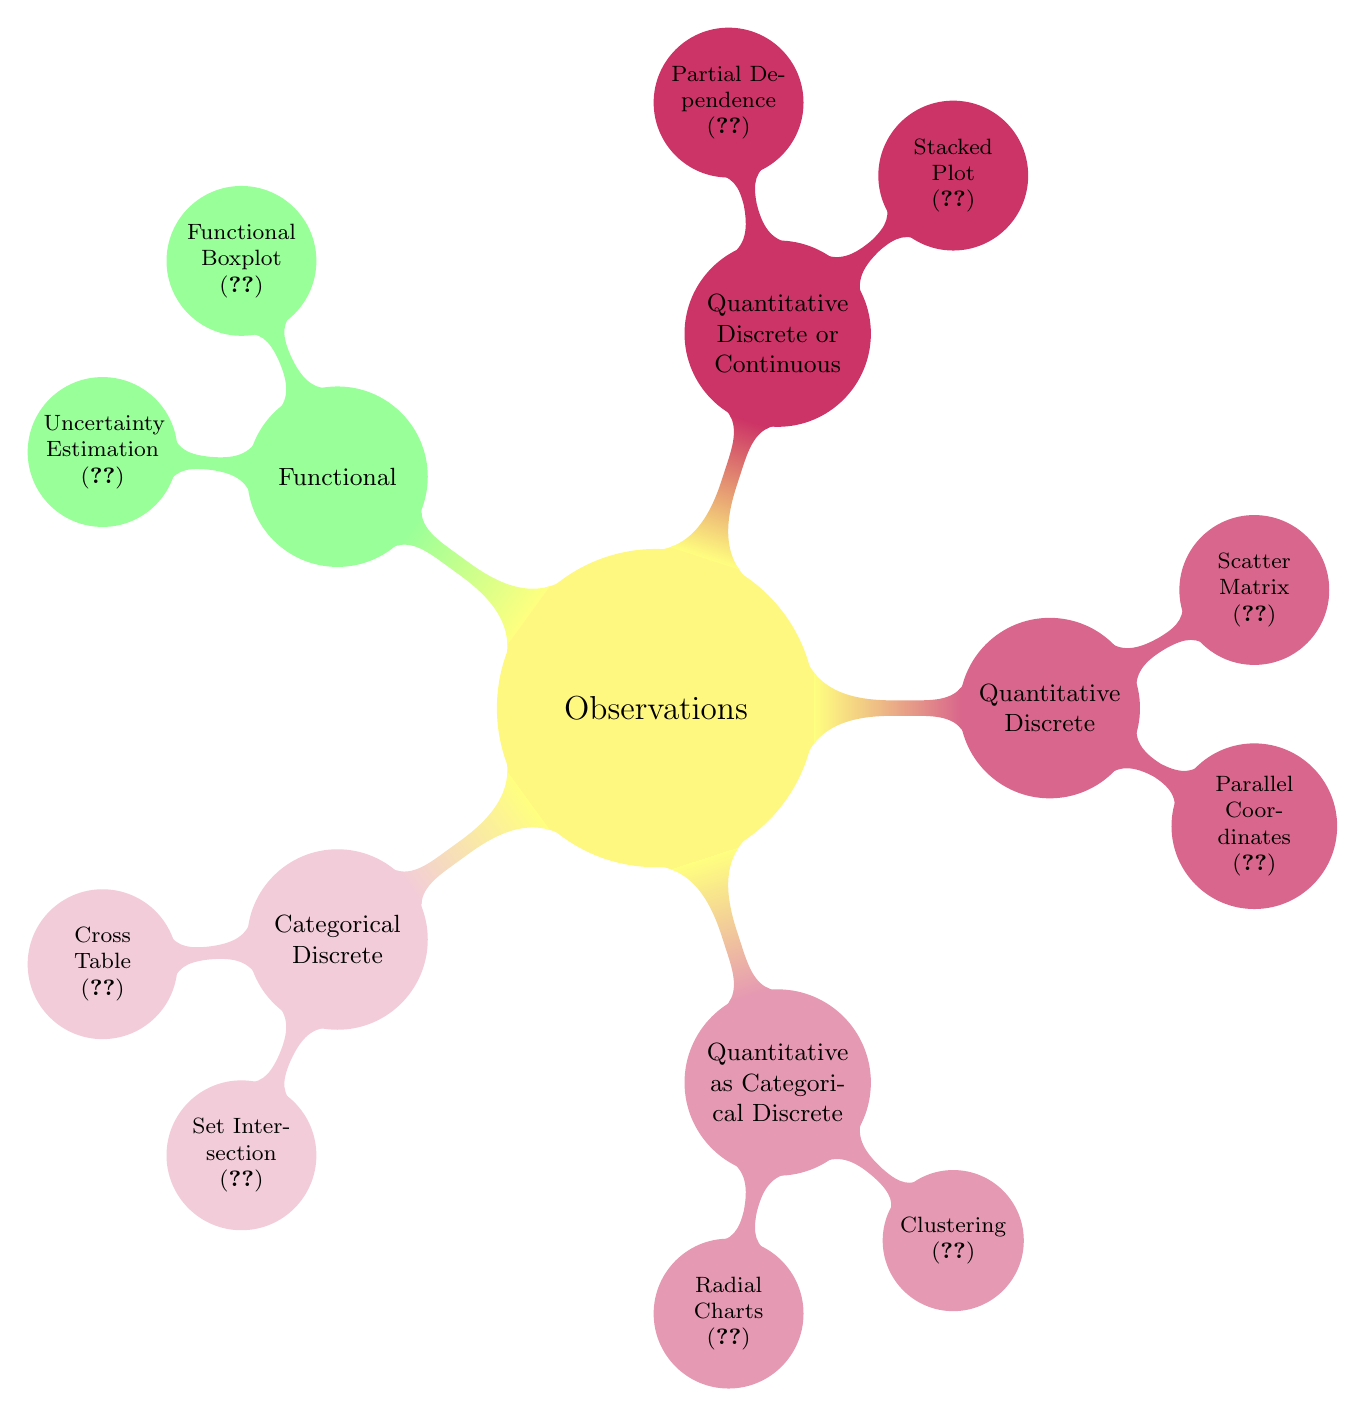
\begin{tikzpicture}[mindmap, grow cyclic, every node/.style=concept, concept color=yellow!50, 
    level 1/.append style={level distance=5cm,sibling angle=72},
    level 2/.append style={level distance=3cm,sibling angle=60},]
    
\node{Observations}
    child[concept color=purple!20]  {node {Categorical Discrete}
            child {node{Cross Table\\(\ref{sec:crosstab})}}
            child {node{Set Intersection\\(\ref{sec:setintersection})}}
            }
    child[concept color=purple!40]  {node {Quantitative as Categorical Discrete}
            child {node{Radial Charts\\(\ref{sec:radial})}}
            child {node{Clustering\\(\ref{sec:cluster})}}
        }
    child[concept color=purple!60]  {node {Quantitative Discrete}
                    child {node{Parallel Coordinates\\(\ref{sec:pcp})}}
                    child {node{Scatter Matrix\\(\ref{sec:condep})}}
        }
    child[concept color=purple!80] {node {Quantitative Discrete or Continuous}
                    child {node {Stacked Plot\\(\ref{sec:stacked})}}
                    child {node{Partial Dependence\\(\ref{sec:pdp})}}
        }
    child[concept color=green!40]  { node {Functional}
        child {node{Functional Boxplot\\(\ref{sec:boxplots})}}
        child {node{Uncertainty Estimation\\(\ref{sec:uncertainty})}}
    }
;
\end{tikzpicture}
\caption{The papers in this survey are organized by the structure of observations and types of measurements in a dataset.}
\label{fig:papermap}
\end{figure}

Although the scatter matrix is limited in the datasets it will work for, there are many other visualization techniques to choose from. As illustrated in figure~\ref{fig:papermap}, this survey provides recommendations for visualization methods based on the structure of the observations and types of measurements in the dataset. This survey presents methods for visualizing conditional dependencies for multivariate datasets with discrete observations and understanding probability distributions for datasets where observations are drawn from a continuous (functional) space. Since there are very few visualizations techniques explicitly designed to show conditional dependency, we include techniques that either suggest a conditional dependency or can be adapted to do so. 

\section{Discrete Observations}
\subfile{sections/section1}
\subfile{sections/section2}
\subfile{sections/section3}
\section{Continuous Observations}
\subfile{sections/section4}
\subfile{sections/section5}

\section{Conclusion}
\label{sec:conclusion}
While this paper described some methods for visualizing conditional dependencies, they are limited. Many visualization techniques only work for a relatively small number of variables, or only when the condition is categorical or temporal. When data has multiple keys, most methods at best can only preserve time or one other one dimensional key. The most promising techniques in the functional space are methods for visualizing distributions and the uncertainty in those visualizations. These techniques could potentially be combined with methods for exploring conditional dependency in discrete and less functional datasets to build new tools for exploring complex data spaces. 


\printbibliography
\end{document}
